%Minor points

%Sample selection: I understand the final sample selection is driven by data availability, but sometimes I was confused by when the policy started and what years are covered by each data source. For example, survey data appear to be available from 2003, and administrative crime records also start in 2003 and run until 2018. Why, then, does the analysis stop in 2012? If this is due to survey availability, that should be made explicit, while the administrative data could still be shown descriptively for the later years. In addition, what distinguishes the municipalities included in the analysis from those excluded? How do early adopters compare to late adopters? For both the survey data and the police records, it would be useful to provide a comparison of characteristics between included and excluded municipalities to give readers confidence that the results are not being driven by sample selection.


Thank you very much for the opportunity to clarify this point. This is related to the availability of data by year and municipality across our two main data sources, and to how the \citet{Callaway} estimator is constructed. When the control group is formed from not-yet-treated units, the estimator only uses data up to the year in which the last treated unit in the data adopts the treatment.

Most outcomes in the paper rely on information from the ENUSC survey, which covers 101 urban municipalities. All of these municipalities were eventually treated except one. Because ENUSC was first conducted in 2003 and not administered in 2004, our main analytical sample includes the 46 urban municipalities that adopted \emph{Plan Cuadrante} between 2005 and 2012---the year in which the last municipality surveyed in ENUSC adopted the program---plus the one never-treated municipality. Even if the ENUSC survey were available after 2012, using these data in the estimation would mean relying only on this single never-treated municipality as the control group for all subsequent periods, which would make the estimates unreliable. We therefore limit the study period in the main analysis to 2003--2012.


Regarding the outcomes constructed from administrative records: these are provided by the Undersecretary for Crime Prevention and are available yearly for all Chilean municipalities---reported crimes from 2002 to 2016, and arrests from 2005 to 2016. This comprehensive coverage results in a much larger number of never-treated units, allowing for a longer estimation period that includes all the data period and municipalities adopting the program up to 2013, when the last Chilean municipality joined \emph{Plan Cuadrante}. In total, we use an analytical sample of 292 municipalities for reported crime and 281 for arrests. For simplicity and symmetry with the ENUSC-based analysis, our main specification nonetheless restricts the event study to 5 pre-treatment and 7 post-treatment periods. We show in Figure \ref{fig:admin_uncapped} in the updated manuscript that the results are very similar when the full set of pre- and post-adoption periods is used instead.

Below we reproduce the relevant paragraphs from the Data subsection of the updated manuscript:

\begin{adjustwidth}{2em}{0em}
We combine administrative and survey data from \emph{Carabineros}, the Undersecretary for Crime Prevention, and the National Institute of Statistics (INE).

\emph{Carabineros} provided information on \emph{Plan Cuadrante} implementation, which we use to define treatment status across municipalities over time. The National Institute of Statistics granted access to the National Survey on Security and Crime (ENUSC), a repeated cross-section first conducted in 2003 and administered annually between October and December since 2005. The survey covers more than 25,000 households across 101 urban municipalities, collecting information on crime victimization, perceptions, trust in police, and household prevention measures over the previous 12 months.\footnote{The survey is administered to a randomly selected household member who must: a) live in the household, b) be 15 years or older, c) not be a domestic worker, and d) not have any disability preventing survey comprehension.}

Our empirical approach excludes always-treated municipalities \citep{Callaway}. Given ENUSC's first implementation in 2003 and absence in 2004, our main sample includes households from 46 urban municipalities that adopted \emph{Plan Cuadrante} between 2005 and 2012 plus one never-treated municipality.\footnote{This sample excludes municipalities adopting \emph{Plan Cuadrante} in 2013 as they are not covered by ENUSC. Also, there is only one never treated municipality covered by ENUSC.} The treated municipalities in this analytical sample account for approximately 27\% of Chile's population.

The Undersecretary for Crime Prevention provided data on the number of reported crimes (2002--2016) and arrests (2005--2016) for all municipalities. This comprehensive coverage allows us to expand the analytical sample: for reported crime, we include all municipalities adopting \emph{Plan Cuadrante} after 2002 together with never-treated municipalities, for a total of 292 municipalities; for arrests, the corresponding sample includes all post-2005 adopters and never-treated municipalities, for a total of 281 municipalities. The treated municipalities in these analytical samples account for over half of Chile's population.

The study period differs across the two data sources, as each covers a different time span and a different set of municipalities. For the ENUSC-based analysis, it is restricted to 2003--2012. The \citet{Callaway} estimator uses not-yet-treated and never-treated municipalities as the comparison group. Since only one municipality in the survey sample is never treated, extending the analysis beyond 2012---the last year in which a municipality surveyed in ENUSC adopts the program---would leave only that single never-treated unit as the comparison group for subsequent periods, making the estimates unreliable. The administrative data, by contrast, cover a large number of never-treated municipalities that can serve as controls throughout the full data period, allowing us to exploit the complete administrative coverage---2002--2016 for reported crime and 2005--2016 for arrests---and to include all municipalities adopting the program from 2003 to 2013, when the last municipality joins \emph{Plan Cuadrante}.

Together, the treated municipalities in our two analytical samples represent substantial shares of the Chilean population---approximately 27\% in the ENUSC-based analysis and over half in the administrative data analysis---and are geographically distributed across the country rather than clustered in a single region. Tables \ref{tab:sum_statsA2} and \ref{tab:sum_statsA3} in Online Appendix \ref{sec:appendixA} and Table \ref{tab:comparing_samples} and Figure \ref{fig:pcsp_maps} in Online Appendix \ref{sec:appendixB} provide a detailed characterization of the treated municipalities in each analytical sample relative to the average Chilean municipality.
\end{adjustwidth}

Note the following footnote to Section 4 in the main manuscript:

\begin{adjustwidth}{2em}{0em}
Online Appendix Figure \ref{fig:admin_uncapped} reports the results for reported crime and arrests using the full set of post-treatment and pre-treatment periods, which are very similar to those presented here.
\end{adjustwidth}

and also the following subsection to Online Appendix C, ``Effects of \emph{Plan Cuadrante} Using the Full Set of Post-treatment and Pre-treatment Periods'':

\begin{adjustwidth}{2em}{0em}
For symmetry with the ENUSC-based analysis, the event studies for reported crime and arrests reported in the main text are restricted to 5 pre-treatment and 7 post-treatment periods. Because the administrative data are available for the full set of Chilean municipalities and therefore include a much larger number of never-treated municipalities than the ENUSC sample, we can estimate these effects over a longer window without exhausting the pool of valid comparison units. Figure \ref{fig:admin_uncapped} reports the effects of \emph{Plan Cuadrante} on reported crime and arrests using the full set of post-treatment and pre-treatment periods rather than capping the event study to the 5 pre-treatment and 7 post-treatment periods used in the main specification. The results are very similar to those presented in Section \ref{main_results}.
\end{adjustwidth}


Finally, we have added the following subsection, ``Characterization of the Analytical Samples,'' to Online Appendix B, comparing the characteristics of the municipalities included in each analytical sample with those excluded from it or always treated:

\begin{adjustwidth}{2em}{0em}
The treated municipalities in our analytical samples are geographically distributed across the country. As shown in Figure \ref{fig:pcsp_maps}, the 46 treated municipalities in the ENUSC-based sample span Chile from north to south, covering a wide range of geographic and socioeconomic contexts, and together account for approximately 27\% of Chile's population. The 96 treated municipalities in the administrative data sample provide even broader national coverage, together accounting for over half of Chile's population.

Table \ref{tab:comparing_samples} characterizes the treated municipalities in each analytical sample relative to all Chilean municipalities (Column 1), all \emph{Plan Cuadrante} municipalities (Column 2), the always-treated municipalities excluded from our estimation samples (Column 3), and never-treated municipalities (Column 6). Columns (4) and (5) report characteristics for the treated municipalities in the ENUSC and administrative data analytical samples respectively. On several dimensions our samples broadly resemble the overall Chilean population: the poverty rate of the 46 treated municipalities in the ENUSC sample (21.7\%) and the 96 treated municipalities in the administrative data sample (24.0\%) are both close to the national average of 23.7\%, and the crime rates of the treated ENUSC municipalities closely track the average across all \emph{Plan Cuadrante} municipalities (2,202 vs.\ 2,132 per 100,000 inhabitants). They do differ on other dimensions---particularly crime rates relative to all Chilean municipalities and population density---but both differences have natural explanations. Higher crime rates are expected because \emph{Plan Cuadrante} exclusively targeted urban municipalities, where crime is more prevalent. The lower-than-average population density in our samples (215 and 135 inhabitants per km$^2$, vs.\ a national mean of 870) reflects the fact that the most densely populated \emph{Plan Cuadrante} municipalities---those of the Santiago metropolitan area---were the earliest adopters of the program and are therefore excluded from our analytical samples as always-treated.
\end{adjustwidth}





\clearpage
\noindent\textbf{Other figures and tables referenced above:}
\vspace{0.5em}

{\renewcommand{\thefigure}{C.8}
\begin{figure}[h!]
    \centering
    \caption{Effects of \emph{Plan Cuadrante} on Reported Crime and Arrests Using the Full Set of Post-treatment and Pre-treatment Periods}
    \label{fig:admin_uncapped}
    \begin{subfigure}{0.495\textwidth}
        \centering
        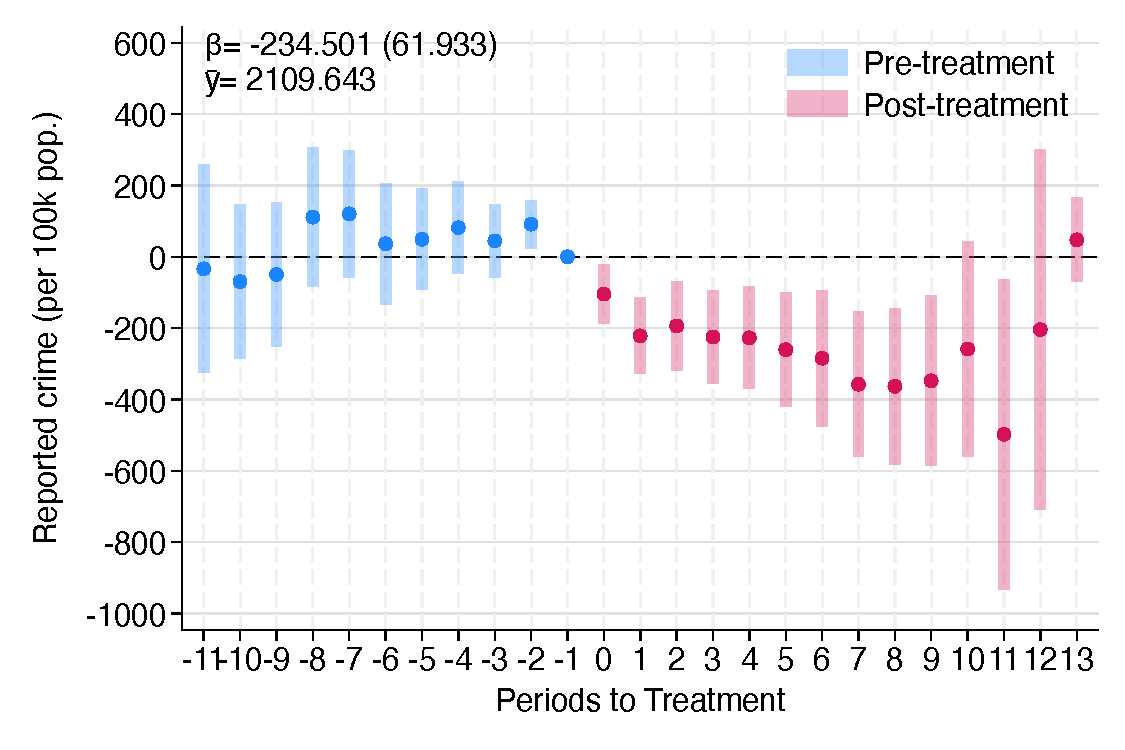
\includegraphics[width=0.98\textwidth]{../manuscript/Graphs/totalreportedcrime_allcomunas_uncapped.pdf}
        \caption{Reported crime per 100k inhabitants}
    \end{subfigure}%
    ~
    \begin{subfigure}{0.495\textwidth}
    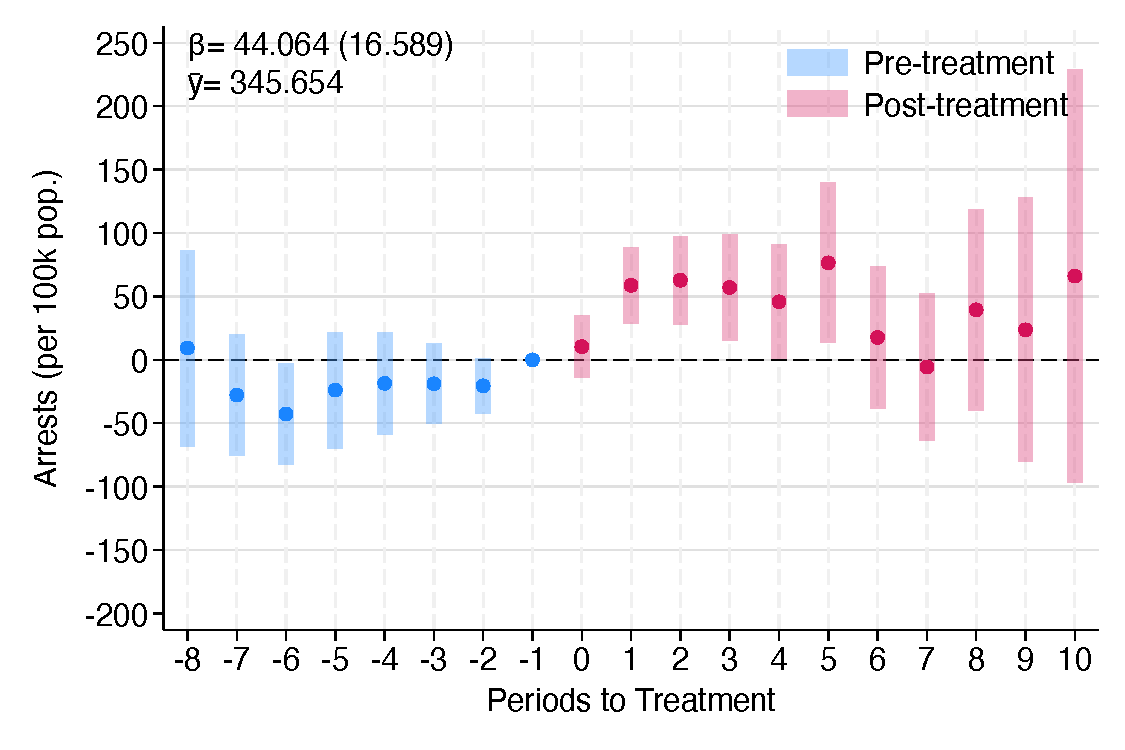
\includegraphics[width=0.98\textwidth]{../manuscript/Graphs/totalarrestscrime_allcomunas_uncapped.pdf}
        \caption{Arrests per 100k inhabitants}
    \end{subfigure}
    \begin{minipage}{\textwidth}
    \footnotesize
   Notes: This figure shows the dynamic effects of \emph{Plan Cuadrante} on the number of crimes reported to the police in the municipality per 100,000 inhabitants (panel a) and on the number of arrests in the municipality per 100,000 inhabitants (panel b), using administrative data. The estimation is conducted using the procedure developed in \citet{Callaway} for difference-in-differences with staggered treatment adoption. The dots in the figure represent the estimated coefficients and the bars behind them 95\% confidence intervals. Standard errors are clustered at the municipality level using the wild bootstrapping procedure. The pooled effect and the mean outcome before the introduction of the treatment are also presented in each panel. Unlike Figure \ref{fig:figure02} in the main text, we do not cap the event study to the same 5 pre-treatment and 6 post-treatment periods used for symmetry with the ENUSC-based analysis. Instead, we exploit the full set of post-treatment and pre-treatment periods. Panel (a) includes 4,371 observations and panel (b) 3,372 observations.
    \end{minipage}
\end{figure}
}

\clearpage

{\renewcommand{\thetable}{A.2}
\begin{table}[H]
\centering
\caption{Summary Statistics -- ENUSC sample}
\label{tab:sum_statsA2}
\begin{threeparttable}
\begin{tabular}{l r r r r r}
\toprule
 & Mean & SD & Min & Max & N \\
\midrule
\multicolumn{6}{@{}l}{\textit{Household}} \\
\quad Socioeconomic status               & 3.58  & 0.73  & 1    & 5    & 99,298 \\
\quad Victimization                    & 0.26  & 0.44  & 0    & 1    & 99,298 \\
\quad Crime perception (neighborhood)  & 0.38  & 0.49  & 0    & 1    & 95,598 \\
\quad Crime perception (municipality)  & 0.66  & 0.48  & 0    & 1    & 96,794 \\
\quad Crime perception (country)       & 0.79  & 0.41  & 0    & 1    & 98,525 \\
\quad Trust in the police              & 0.44  & 0.50  & 0    & 1    & 51,445 \\
\quad Investment in security measures  & 0.21  & 0.40  & 0    & 1    & 99,298 \\
\quad \emph{Plan Cuadrante} (year)                  & 2007  & 1.85  & 2005 & 2012 & 97,847 \\
\addlinespace
\multicolumn{6}{@{}l}{\textit{Household member interviewed}} \\
\quad Female                      & 0.55  & 0.50  & 0  & 1  & 99,298 \\
\quad Age                         & 43.87 & 17.95 & 15 & 99 & 99,298 \\
\quad Primary school attendance   & 0.98  & 0.14  & 0  & 1  & 99,298 \\
\quad Secondary school attendance & 0.72  & 0.45  & 0  & 1  & 99,298 \\
\quad University attendance       & 0.20  & 0.40  & 0  & 1  & 99,298 \\
\bottomrule
\end{tabular}
\begin{tablenotes}[flushleft]
\footnotesize
\item Note: This table presents summary statistics from the ENUSC sample, covering the 47 municipalities used in the survey-based analysis (46 that adopted \emph{Plan Cuadrante} between 2005 and 2012 plus one never-treated municipality). Socioeconomic status is a 1 to 5 measure produced by ENUSC surveys and based on self-reported socioeconomic strata, being 1 the highest ranked and 5 the lowest. Crime perception is equal to 1 if the interviewed person reports that crime has increased in the last 12 months. The \emph{Plan Cuadrante} (year) row is computed over treated municipalities only.
\end{tablenotes}
\end{threeparttable}
\end{table}
}

\clearpage

{\renewcommand{\thetable}{A.3}
\begin{table}[H]
\centering
\caption{Summary Statistics -- Administrative municipality level sample}
\label{tab:sum_statsA3}
\begin{threeparttable}
\begin{tabular}{l r r r r r}
\toprule
 & Mean & SD & Min & Max & N \\
\midrule
\multicolumn{6}{@{}l}{\textit{Panel A. Reported-crime sample (292 municipalities)}} \\
\quad Reported crime (per 100k pop.)            & 1,732.39 & 1,036.68 & 0.00   & 11,434.40 & 4,371 \\
\quad Arrests (per 100k pop.)                   & 332.07   & 271.75   & 0.00   & 1,712.30  & 3,504 \\
\quad Poverty rate (\%)                         & 25.74    & 9.72     & 5.65   & 58.33     & 3,720 \\
\quad Pop.\ density (pop./km\textsuperscript{2}) & 63.51   & 140.47   & 0.09   & 1,109.58  & 4,065 \\
\quad \emph{Plan Cuadrante} (year)                     & 2010     & 2.82     & 2003   & 2013      & 1,440 \\
\addlinespace
\multicolumn{6}{@{}l}{\textit{Panel B. Arrests sample (281 municipalities)}} \\
\quad Reported crime (per 100k pop.)            & 1,684.74 & 1,014.67 & 0.00   & 11,434.40 & 4,209 \\
\quad Arrests (per 100k pop.)                   & 313.21   & 251.23   & 0.00   & 1,712.30  & 3,372 \\
\quad Poverty rate (\%)                         & 26.01    & 9.72     & 5.65   & 58.33     & 3,570 \\
\quad Pop.\ density (pop./km\textsuperscript{2}) & 57.90   & 127.30   & 0.09   & 1,109.58  & 3,900 \\
\quad \emph{Plan Cuadrante} (year)                     & 2010     & 2.26     & 2006   & 2013      & 1,275 \\
\bottomrule
\end{tabular}
\begin{tablenotes}[flushleft]
\footnotesize
\item Note: The table reports municipality-level summary statistics for the two administrative estimation samples used in the paper. Panel A covers the 292 municipalities in the reported-crime sample (municipalities adopting \emph{Plan Cuadrante} from 2003 onward plus never-treated); Panel B the 281 municipalities in the arrests sample (adopters from 2006 onward plus never-treated --- municipalities adopting in 2005 are excluded because arrest data begin that year, leaving no pre-treatment period). Reported crime and arrests are measured per 100,000 inhabitants over 2002--2016 and 2005--2016, respectively. Minimum reported crime and arrests of zero correspond to tiny, remote never-treated comunas (e.g., Juan Fernández, Cabo de Hornos). The \emph{Plan Cuadrante} (year) row is computed over treated municipalities only. Data from the Undersecretary for Crime Prevention.
\end{tablenotes}
\end{threeparttable}
\end{table}
}

\clearpage

{\renewcommand{\thefigure}{B.1}
\begin{figure}[h!]
    \centering
    \caption{Geographic Distribution of \emph{Plan Cuadrante}}
    \label{fig:pcsp_maps}
    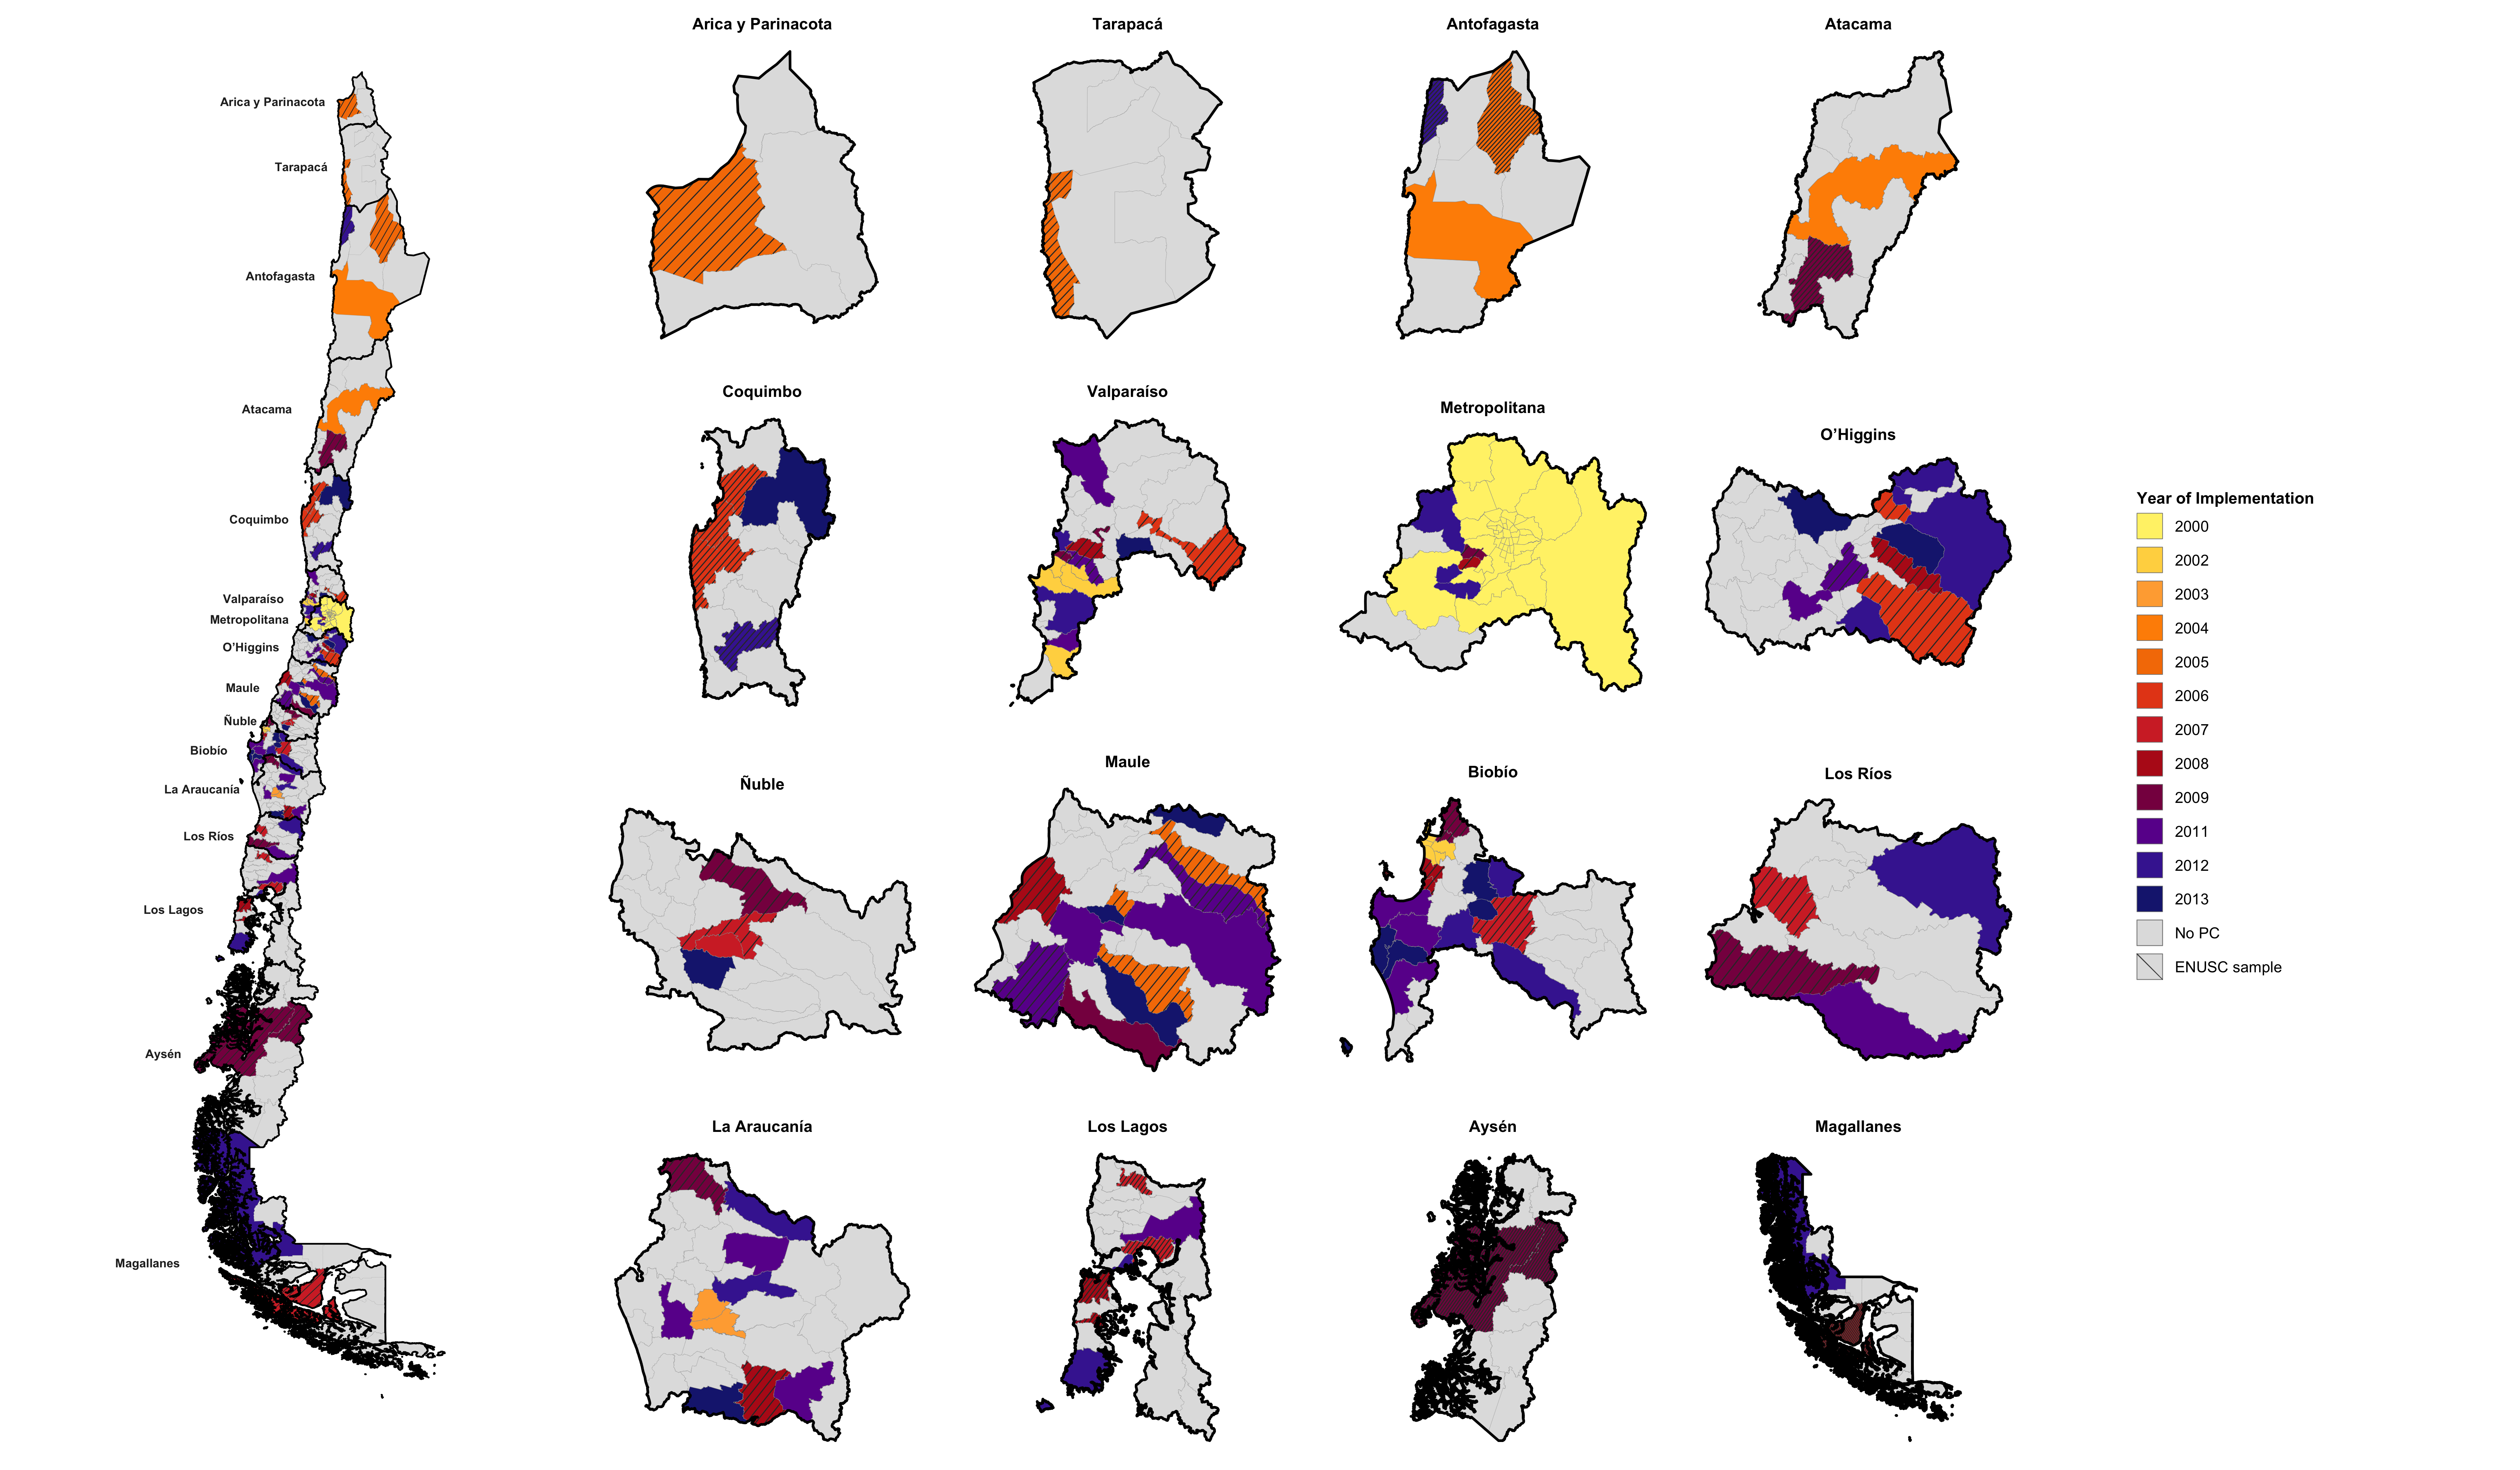
\includegraphics[width=\textwidth]{../manuscript/Graphs/mapa_PCSP_Chile_combinado.png}
    \begin{minipage}{0.95\textwidth}
    \footnotesize
    Notes: This figure shows the spatial rollout of \emph{Plan Cuadrante} across Chilean municipalities. The national map (left) is displayed alongside the 16 regional maps (right) for closer inspection. The color of each treated municipality indicates its year of program adoption, ranging from 2000 (lightest) to 2013 (darkest), following the legend. Municipalities shown in light grey were never treated under PC. Diagonal hatching identifies the 46 treated municipalities in the analytical sample used to estimate the effects on ENUSC outcomes.
    \end{minipage}
\end{figure}
}

\clearpage

{\renewcommand{\thetable}{B.1}
\begin{table}[H]
\caption{Baseline characteristics by subsample}
\label{tab:comparing_samples}
\begin{center}
\resizebox{\textwidth}{!}{
\begin{threeparttable}
\begin{tabular}{l cccccc}
\toprule
&  & \multicolumn{4}{c}{PC municipalities}  & \\
\cmidrule(lr){3-6}
& (1) & (2) & (3) & (4) & (5) & (6) \\
& All & All PC & Always- & Treated & Treated & Never- \\
& municipalities & municipalities & treated & ENUSC & admin.\ data & treated \\
\midrule
Reported crime (per 100k pop.) &     1,650.23 &     2,132.29 &     2,437.25 &     2,202.06 &     1,976.59 &     1,282.47 \\
Arrests (per 100k pop.)        &       267.62     &       442.08     &       606.01     &       459.05     &       358.11     &       134.11     \\
Poverty rate (\%)              &        23.73     &        20.50     &        14.88     &        21.73     &        23.96     &        26.82     \\
Pop.\ density (pop./km$^2$)   &       870.28 &     1,904.14 &     4,593.32 &       215.52 &       134.50 &        27.02 \\
Population                     &    57,857.22         &   117,975.43         &   187,558.74         &   113,079.74         &    81,532.84         &    11,612.44         \\
\midrule
Municipalities                 &          346            &          150            &           58            &           46            &           96            &          196            \\
\bottomrule
\end{tabular}
\begin{tablenotes}[flushleft]
\footnotesize{\item Note: Reported crime, poverty rate, population density, and population are measured as of 2003; arrests are measured as of 2005, the first year for which arrest data are available. Column (1) includes all municipalities in Chile. Column (2) includes all PC municipalities. Column (3) restricts to municipalities that adopted \emph{Plan Cuadrante} before 2005, the always-treated in our sample, which are therefore excluded from our estimation samples (as depicted in Figure 1, panel (a)). Column (4) restricts to treated municipalities in the analytical sample using the ENUSC data. Column (5) restricts to treated municipalities included in the analytical sample using the administrative data. Column (6) includes never-treated municipalities.}
\end{tablenotes}
\end{threeparttable}}
\end{center}
\end{table}
}

\clearpage
